\subsubsection{Thiết kế giao diện}
Mục tiêu của nhóm là xây dựng một giao diện hiện đại, thân thiện, giúp người dùng dễ dàng tiếp cận các tính năng phức tạp như "Gợi ý lịch trình bằng AI"\ hay "Tra cứu đánh giá cộng đồng"\ một cách mượt mà nhất.

Thiết kế của TravelEZ tuân thủ các nguyên tắc về sự tối giản và tính nhất quán, ưu tiên hiển thị hình ảnh điểm đến chất lượng cao để khơi gợi cảm hứng du lịch. Đồng thời, hệ thống điều hướng được tối ưu hóa để người dùng có thể thao tác nhanh chóng chỉ với một tay, phù hợp với thói quen sử dụng thiết bị di động khi đang di chuyển.

Hệ thống TravelEZ bao gồm các màn hình chức năng cốt lõi được thiết kế để tối ưu hóa luồng trải nghiệm người dùng từ khâu lên ý tưởng, lập kế hoạch đến khi thực hiện chuyến đi.
\begin{enumerate}
    \item \textbf{Trang chủ:} Cung cấp cái nhìn tổng quan về các tính năng chính của ứng dụng, hiển thị các điểm đến nổi bật, các gợi ý nhanh dựa trên xu hướng hiện tại và lối tắt truy cập nhanh vào tính năng lập kế hoạch AI (Hình \ref{fig:homepage}).
    \item \textbf{Lập kế hoạch chuyến đi bằng AI:} Giao diện tập trung vào việc thu thập các dữ liệu đầu vào quan trọng từ người dùng bao gồm: Điểm đến, Thời gian, Ngân sách dự kiến, Sở thích cá nhân (ẩm thực, văn hóa, mạo hiểm...), và Số lượng thành viên. Sau khi người dùng nhập dữ liệu, hệ thống sẽ hiển thị lịch trình được AI đề xuất một cách trực quan, kèm theo các tùy chọn chỉnh sửa linh hoạt (Hình \ref{fig:planning-1}, \ref{fig:planning-2}, \ref{fig:planning-3}, \ref{fig:planning-4}, \ref{fig:planning-5}, \ref{fig:planning-6}).
    \item \textbf{Xem chi tiết lịch trình:} Giao diện trình bày chi tiết từng ngày trong lịch trình đã được AI đề xuất, bao gồm các hoạt động, địa điểm tham quan, thời gian di chuyển và các ghi chú quan trọng. Người dùng có thể dễ dàng điều chỉnh lịch trình hoặc thêm ghi chú cá nhân (Hình \ref{fig:itinerary}).
    \item \textbf{Quản lý chuyến đi}: Nơi lưu trữ và quản lý tất cả các hành trình của người dùng (Hình \ref{fig:trips}).
    \item \textbf{Khám phá điểm đến}: Giao diện trình bày thông tin chi tiết về các điểm đến và các gợi ý hoạt động nổi bật (Hình \ref{fig:discovery}).
    \item \textbf{Danh sách địa điểm}: Hiển thị danh sách các địa điểm thuộc một khu vực hoặc một danh mục cụ thể (Khách sạn, Nhà hàng, Vui chơi). Hỗ trợ các bộ lọc nâng cao theo giá cả, đánh giá sao, và khoảng cách để người dùng dễ dàng sàng lọc (Hình \ref{fig:city}).
    \item \textbf{Chi tiết địa điểm}: Cung cấp thông tin chi tiết về địa điểm bao gồm mô tả, hình ảnh, đánh giá từ cộng đồng, và các tùy chọn đặt chỗ trực tiếp (Hình \ref{fig:poi}).
    \item \textbf{Đánh giá}: Giao diện cho phép người dùng đọc và viết đánh giá về các địa điểm họ đã trải nghiệm, giúp xây dựng cộng đồng chia sẻ thông tin du lịch (Hình \ref{fig:review}).
\end{enumerate}

\begin{figure}[H]
    \centering
    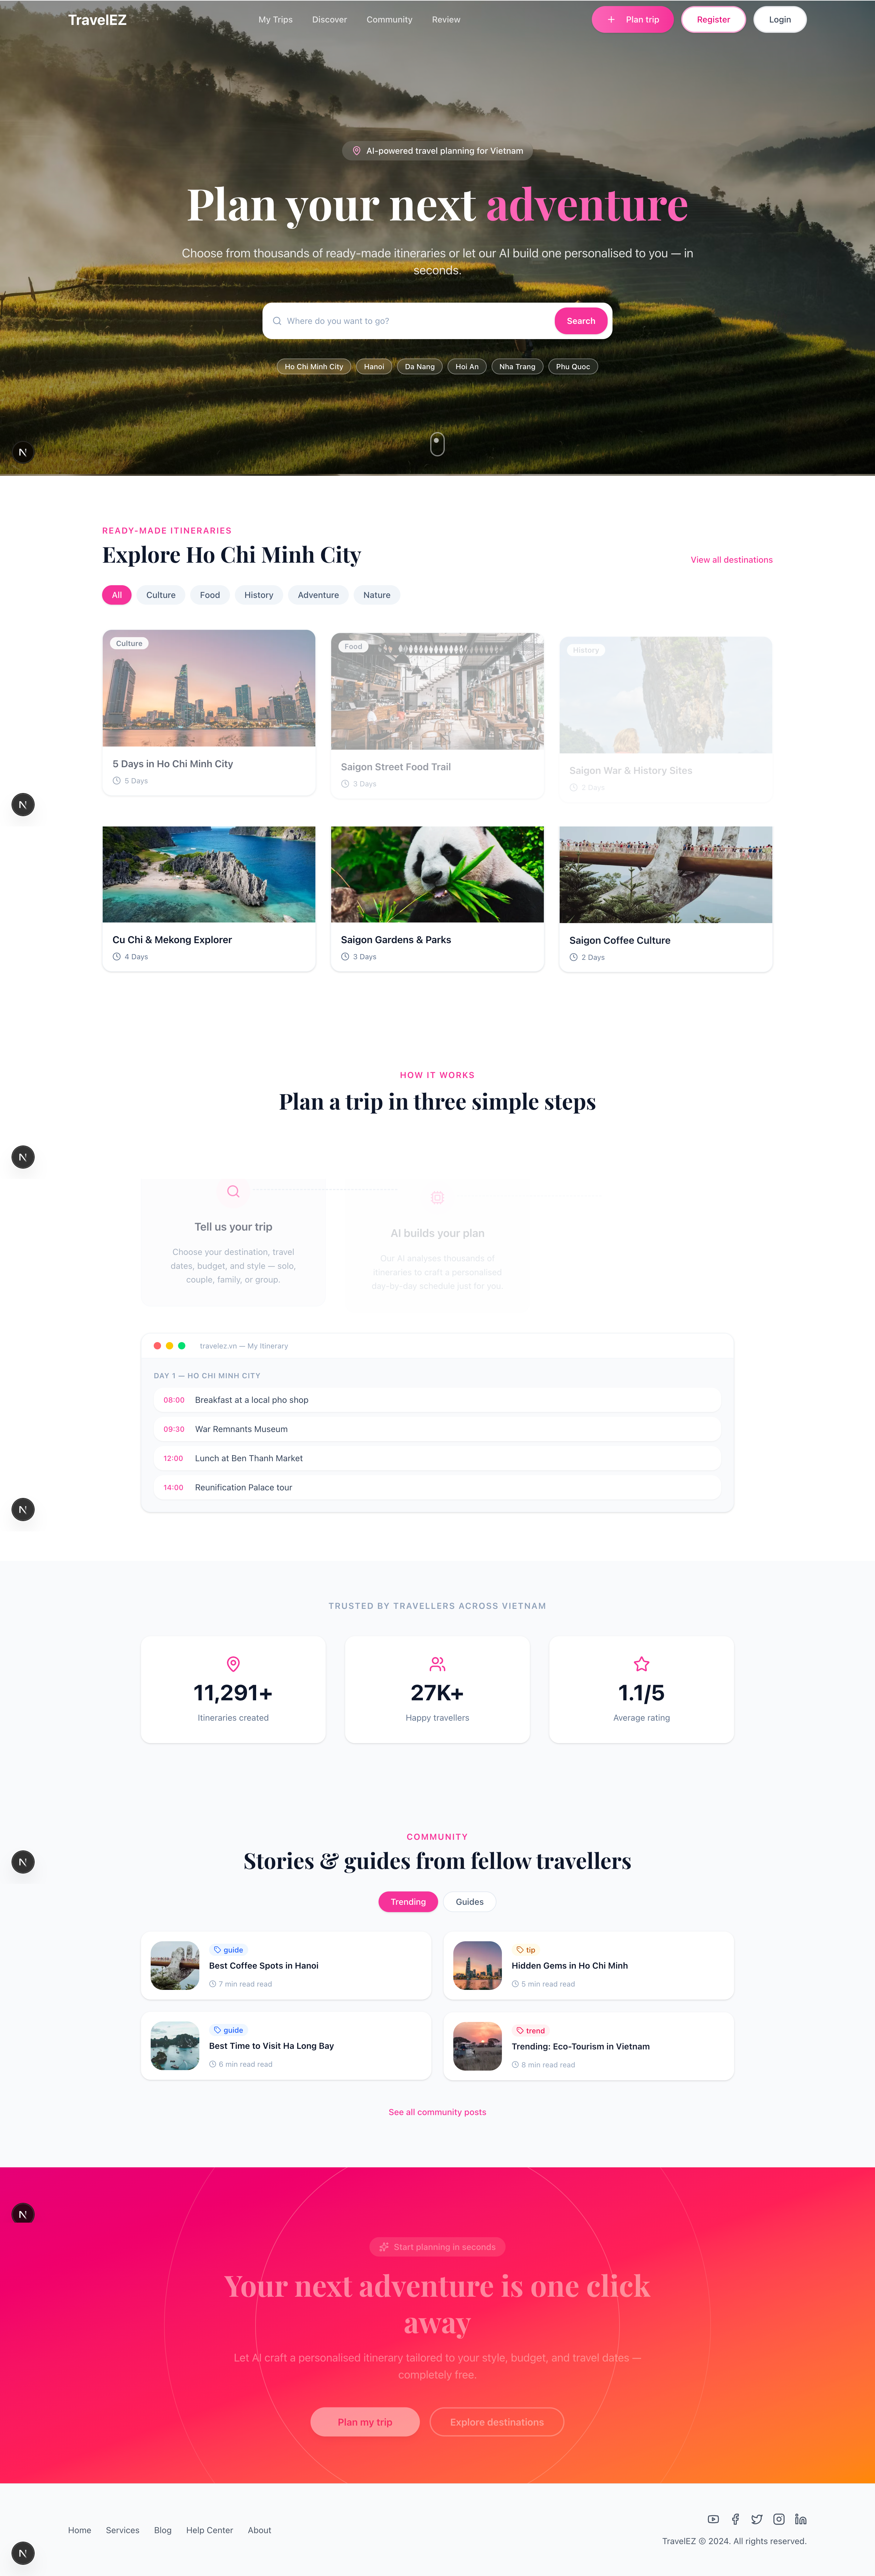
\includegraphics[
        height=1\textheight,
        keepaspectratio
    ]{Images/7. System Design/UI design/home.png}
    \caption{Trang chủ của ứng dụng TravelEZ}
    \label{fig:homepage}
\end{figure}

\begin{figure}[H]
    \centering
    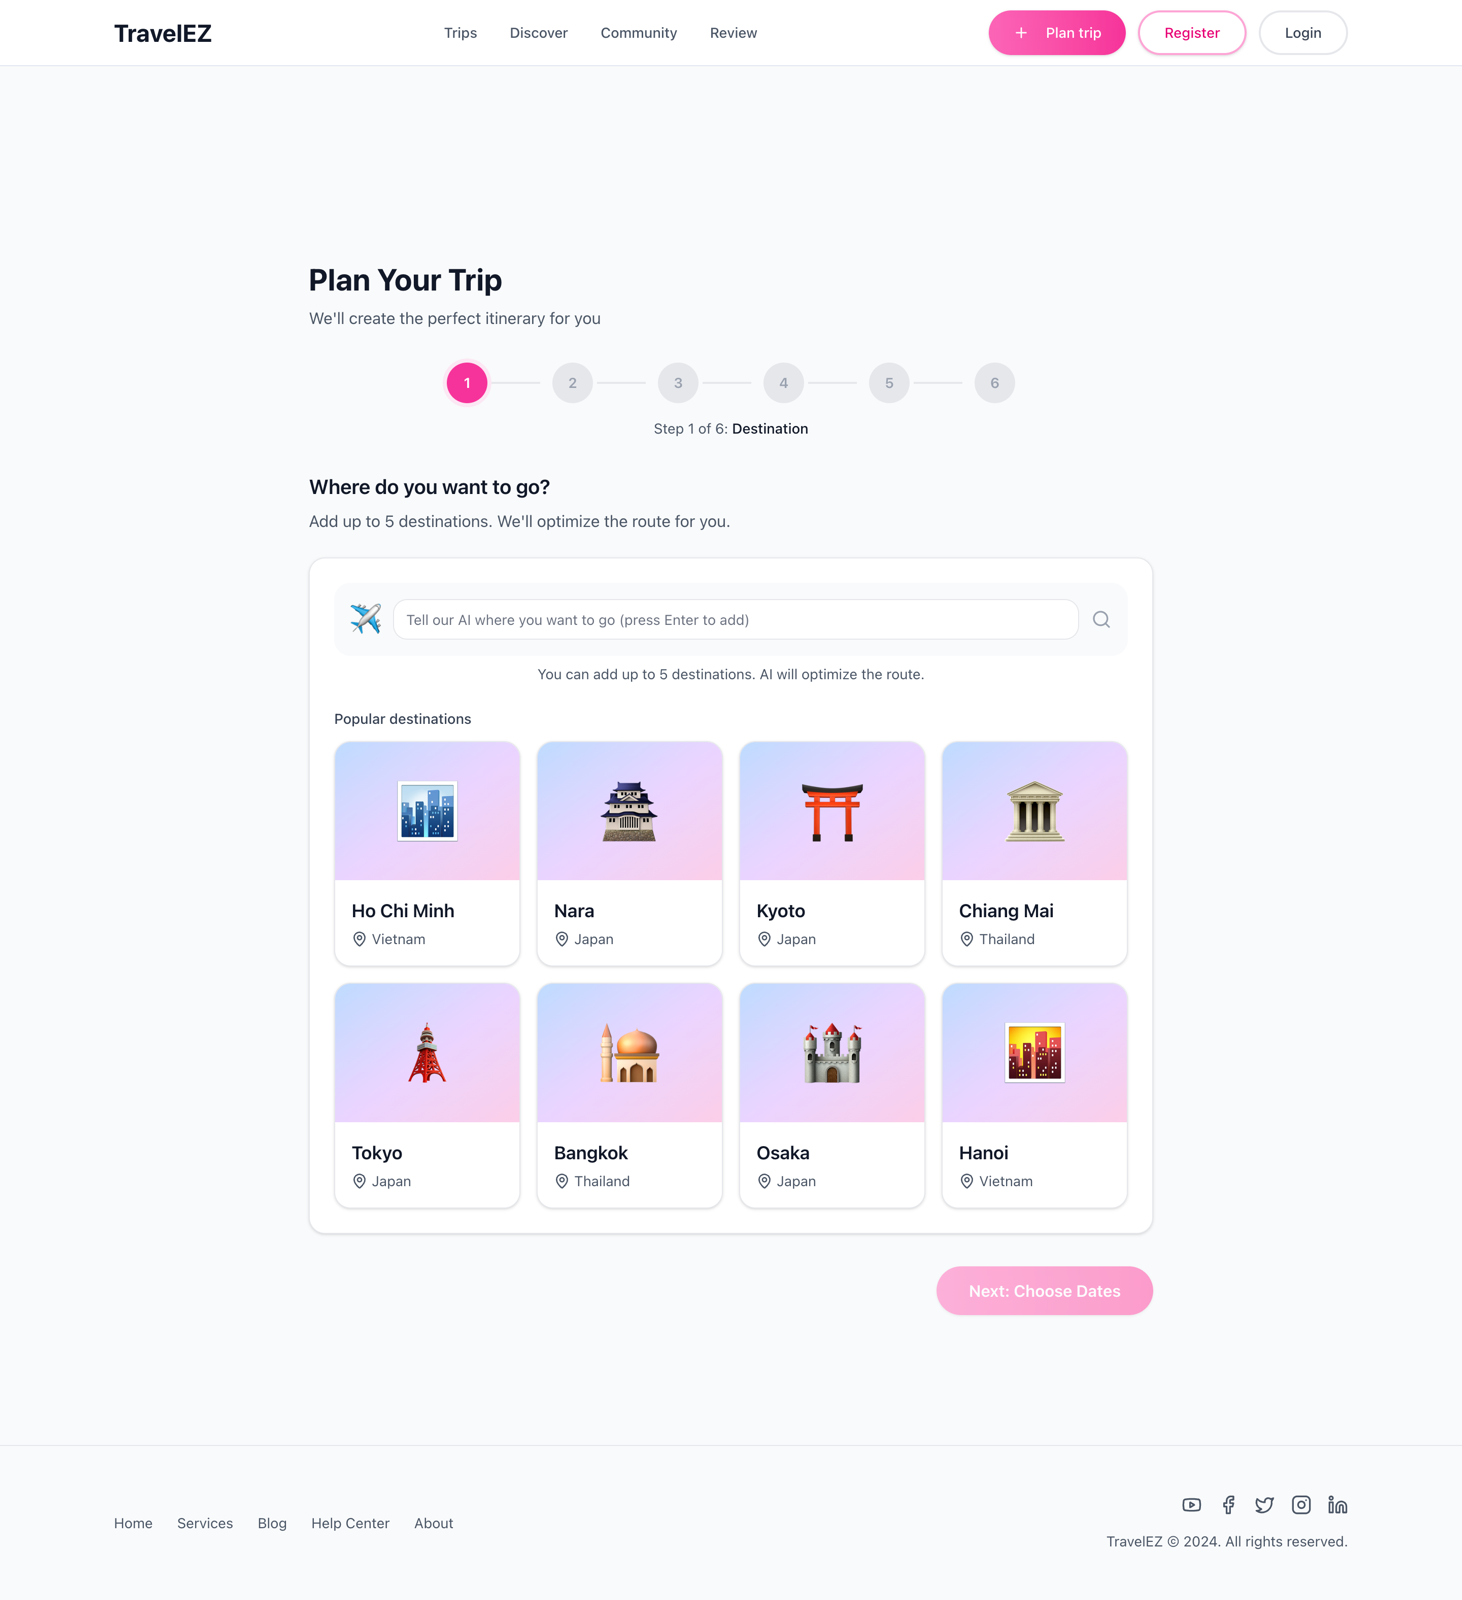
\includegraphics[
        width=1\textwidth
    ]{Images/7. System Design/UI design/planning-1.png}
    \caption{Trang lập kế hoạch chuyến đi bằng AI (bước 1 - Chọn địa điểm)}
    \label{fig:planning-1}
\end{figure}

\begin{figure}[H]
    \centering
    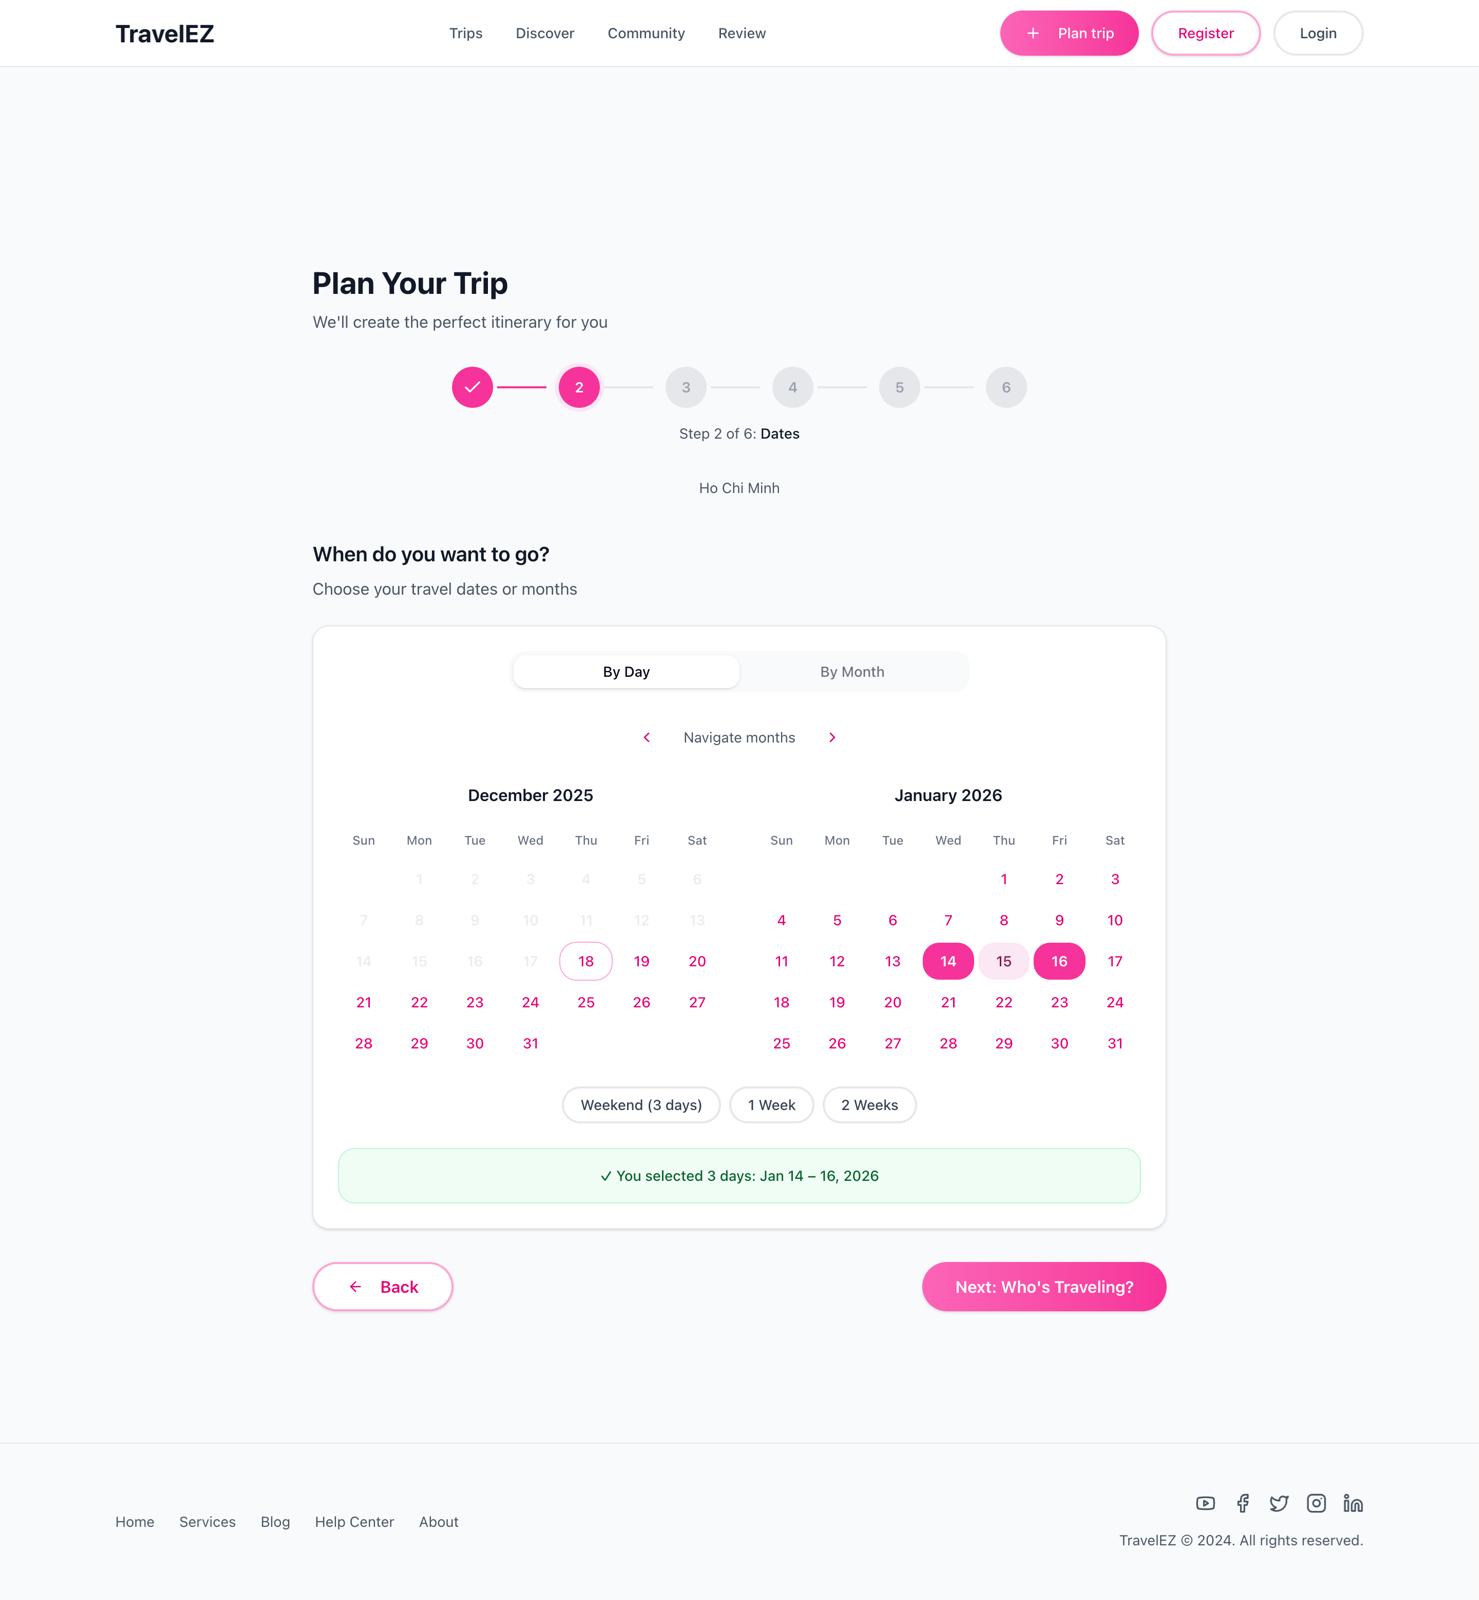
\includegraphics[
        width=1\textwidth
    ]{Images/7. System Design/UI design/planning-2.png}
    \caption{Trang lập kế hoạch chuyến đi bằng AI (bước 2 - Chọn thời gian)}
    \label{fig:planning-2}
\end{figure}

\begin{figure}[H]
    \centering
    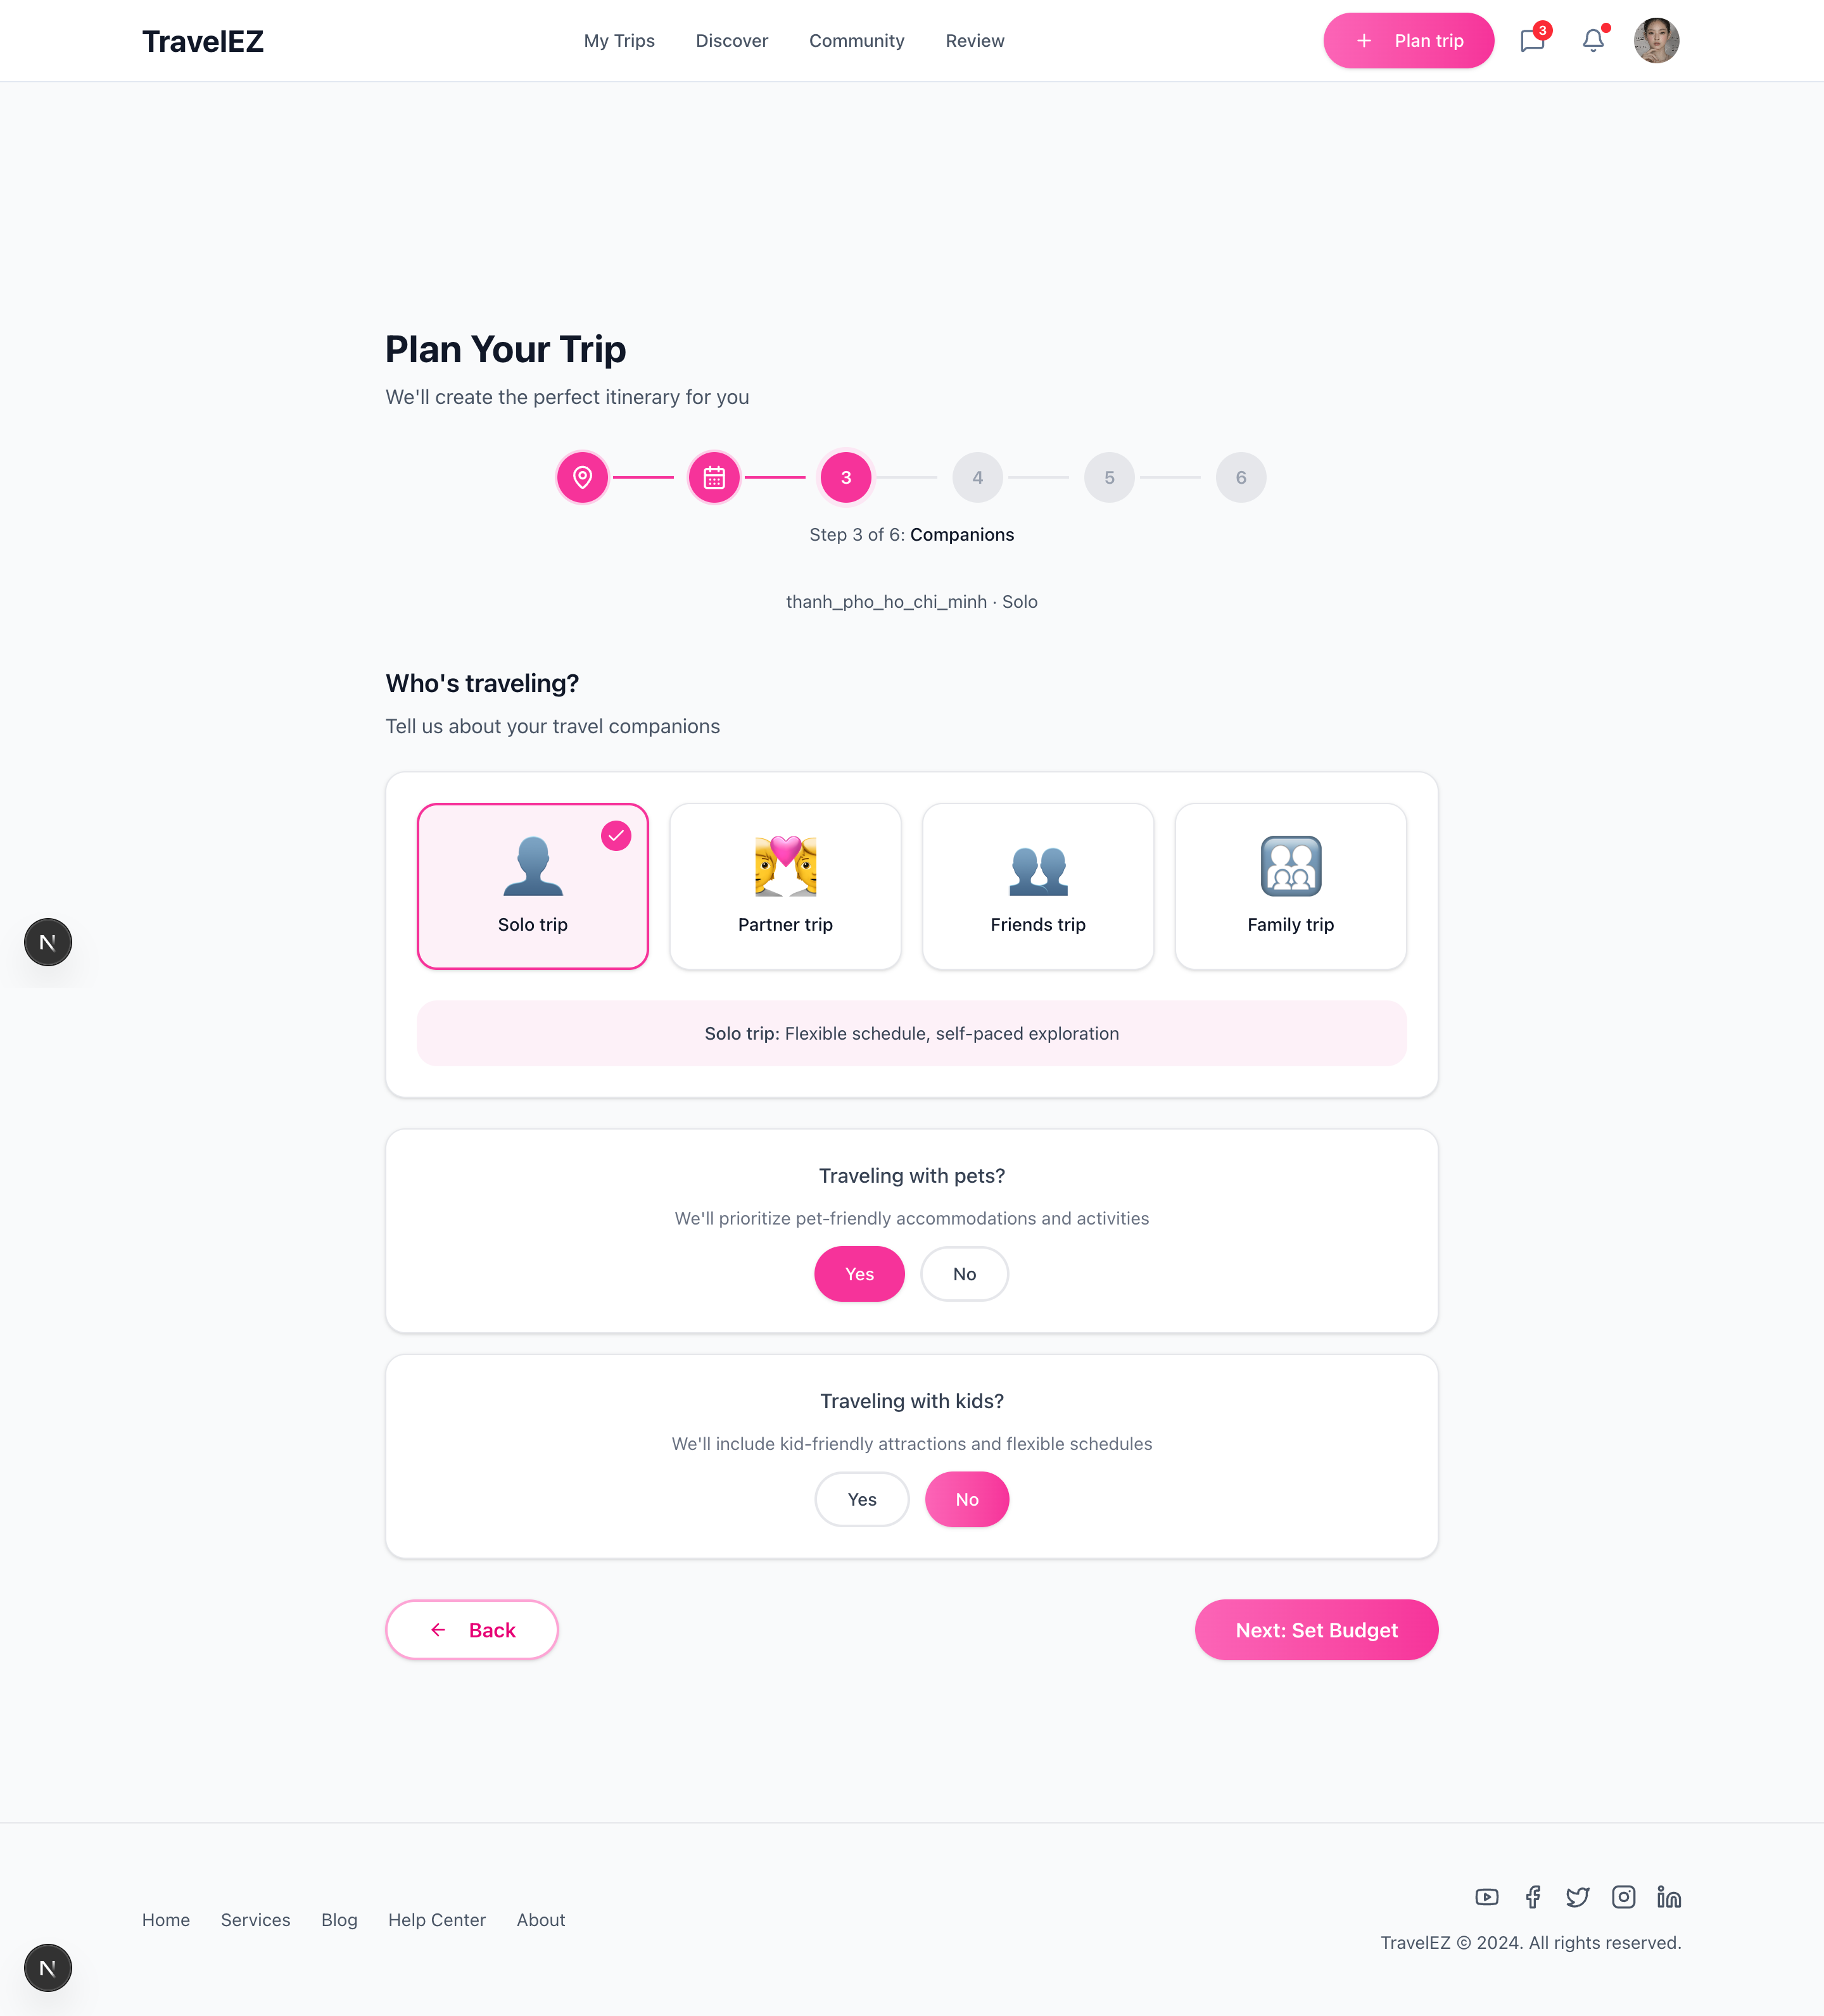
\includegraphics[
        width=1\textwidth
    ]{Images/7. System Design/UI design/planning-3.png}
    \caption{Trang lập kế hoạch chuyến đi bằng AI (bước 3 - Chọn nhu cầu)}
    \label{fig:planning-3}
\end{figure}

\begin{figure}[H]
    \centering
    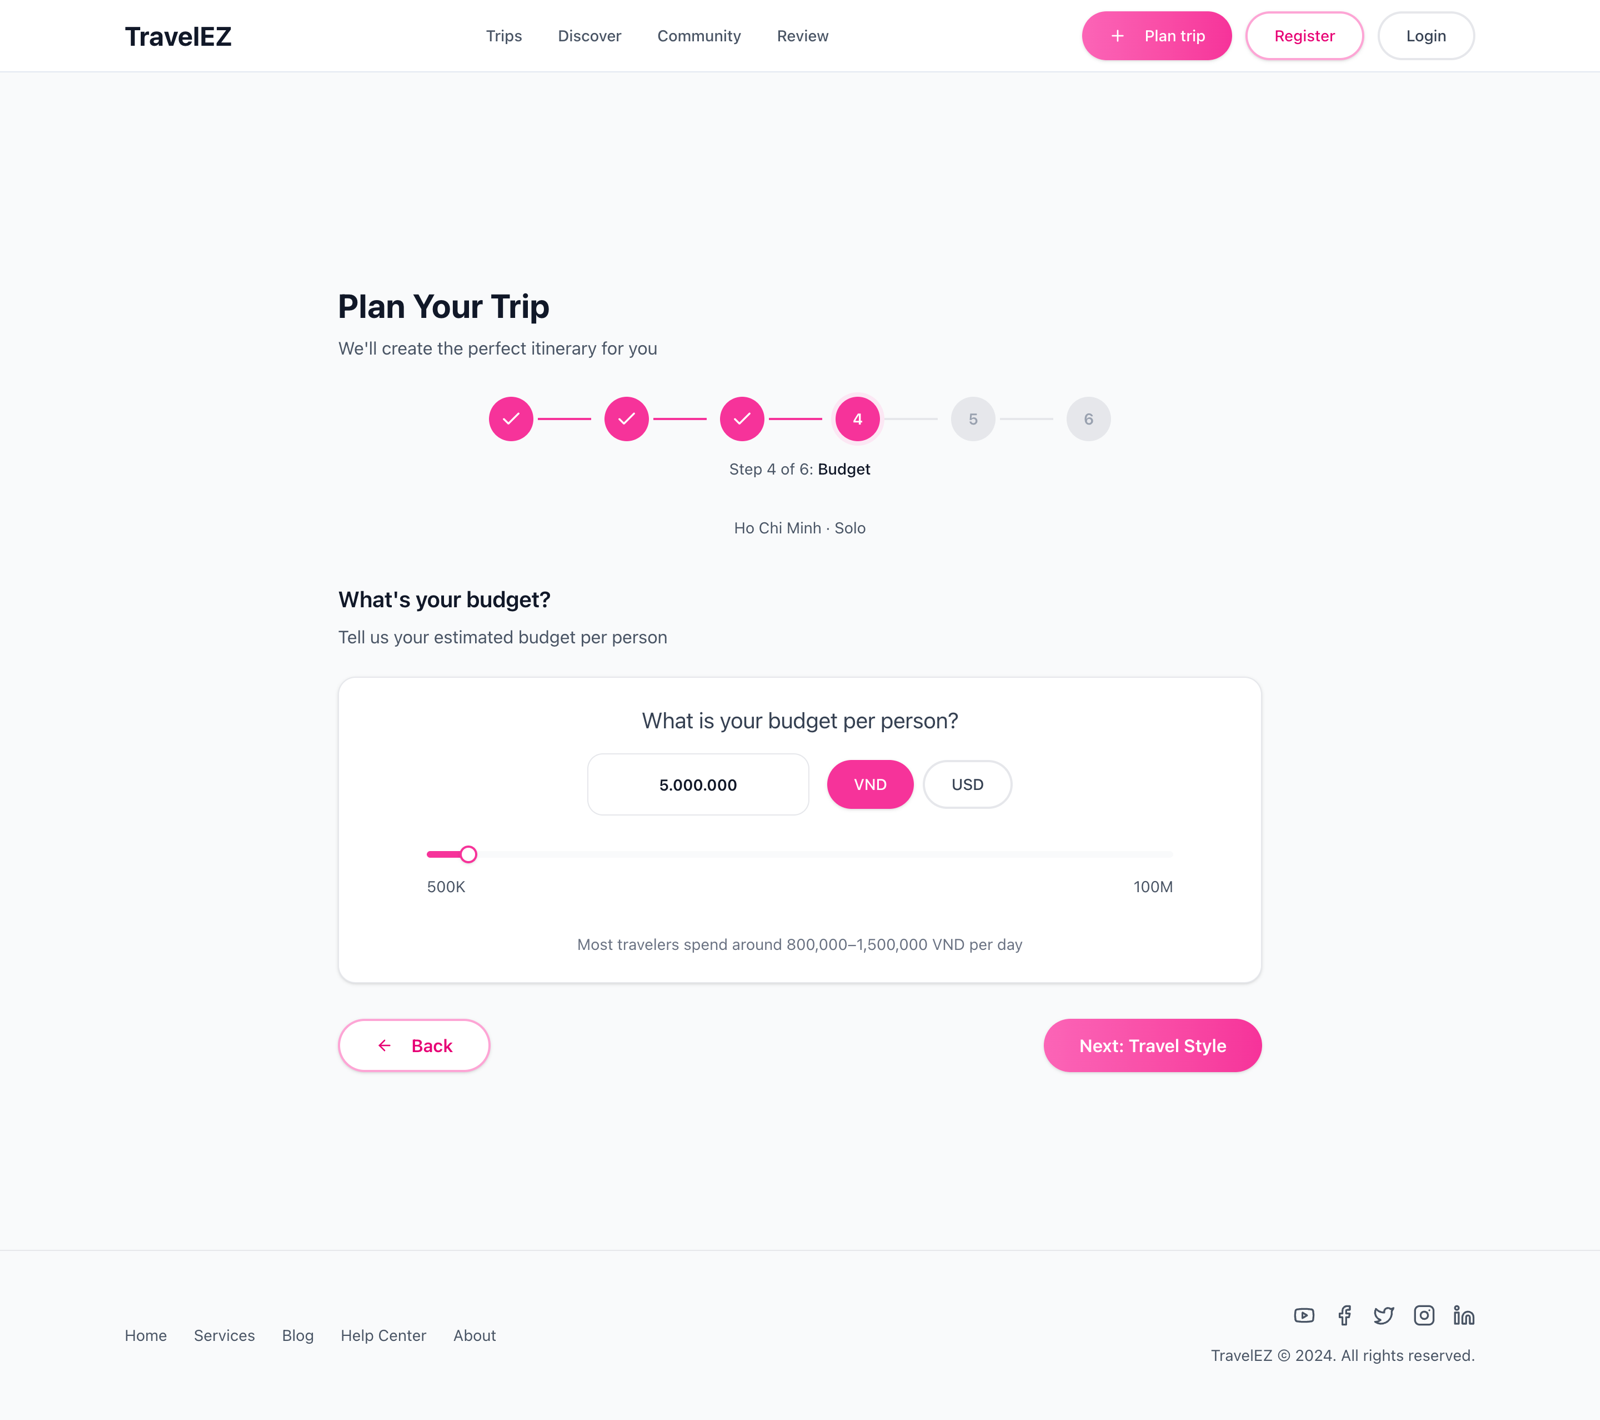
\includegraphics[
        width=1\textwidth
    ]{Images/7. System Design/UI design/planning-4.png}
    \caption{Trang lập kế hoạch chuyến đi bằng AI (bước 4 - Chọn ngân sách)}
    \label{fig:planning-4}
\end{figure}

\begin{figure}[H]
    \centering
    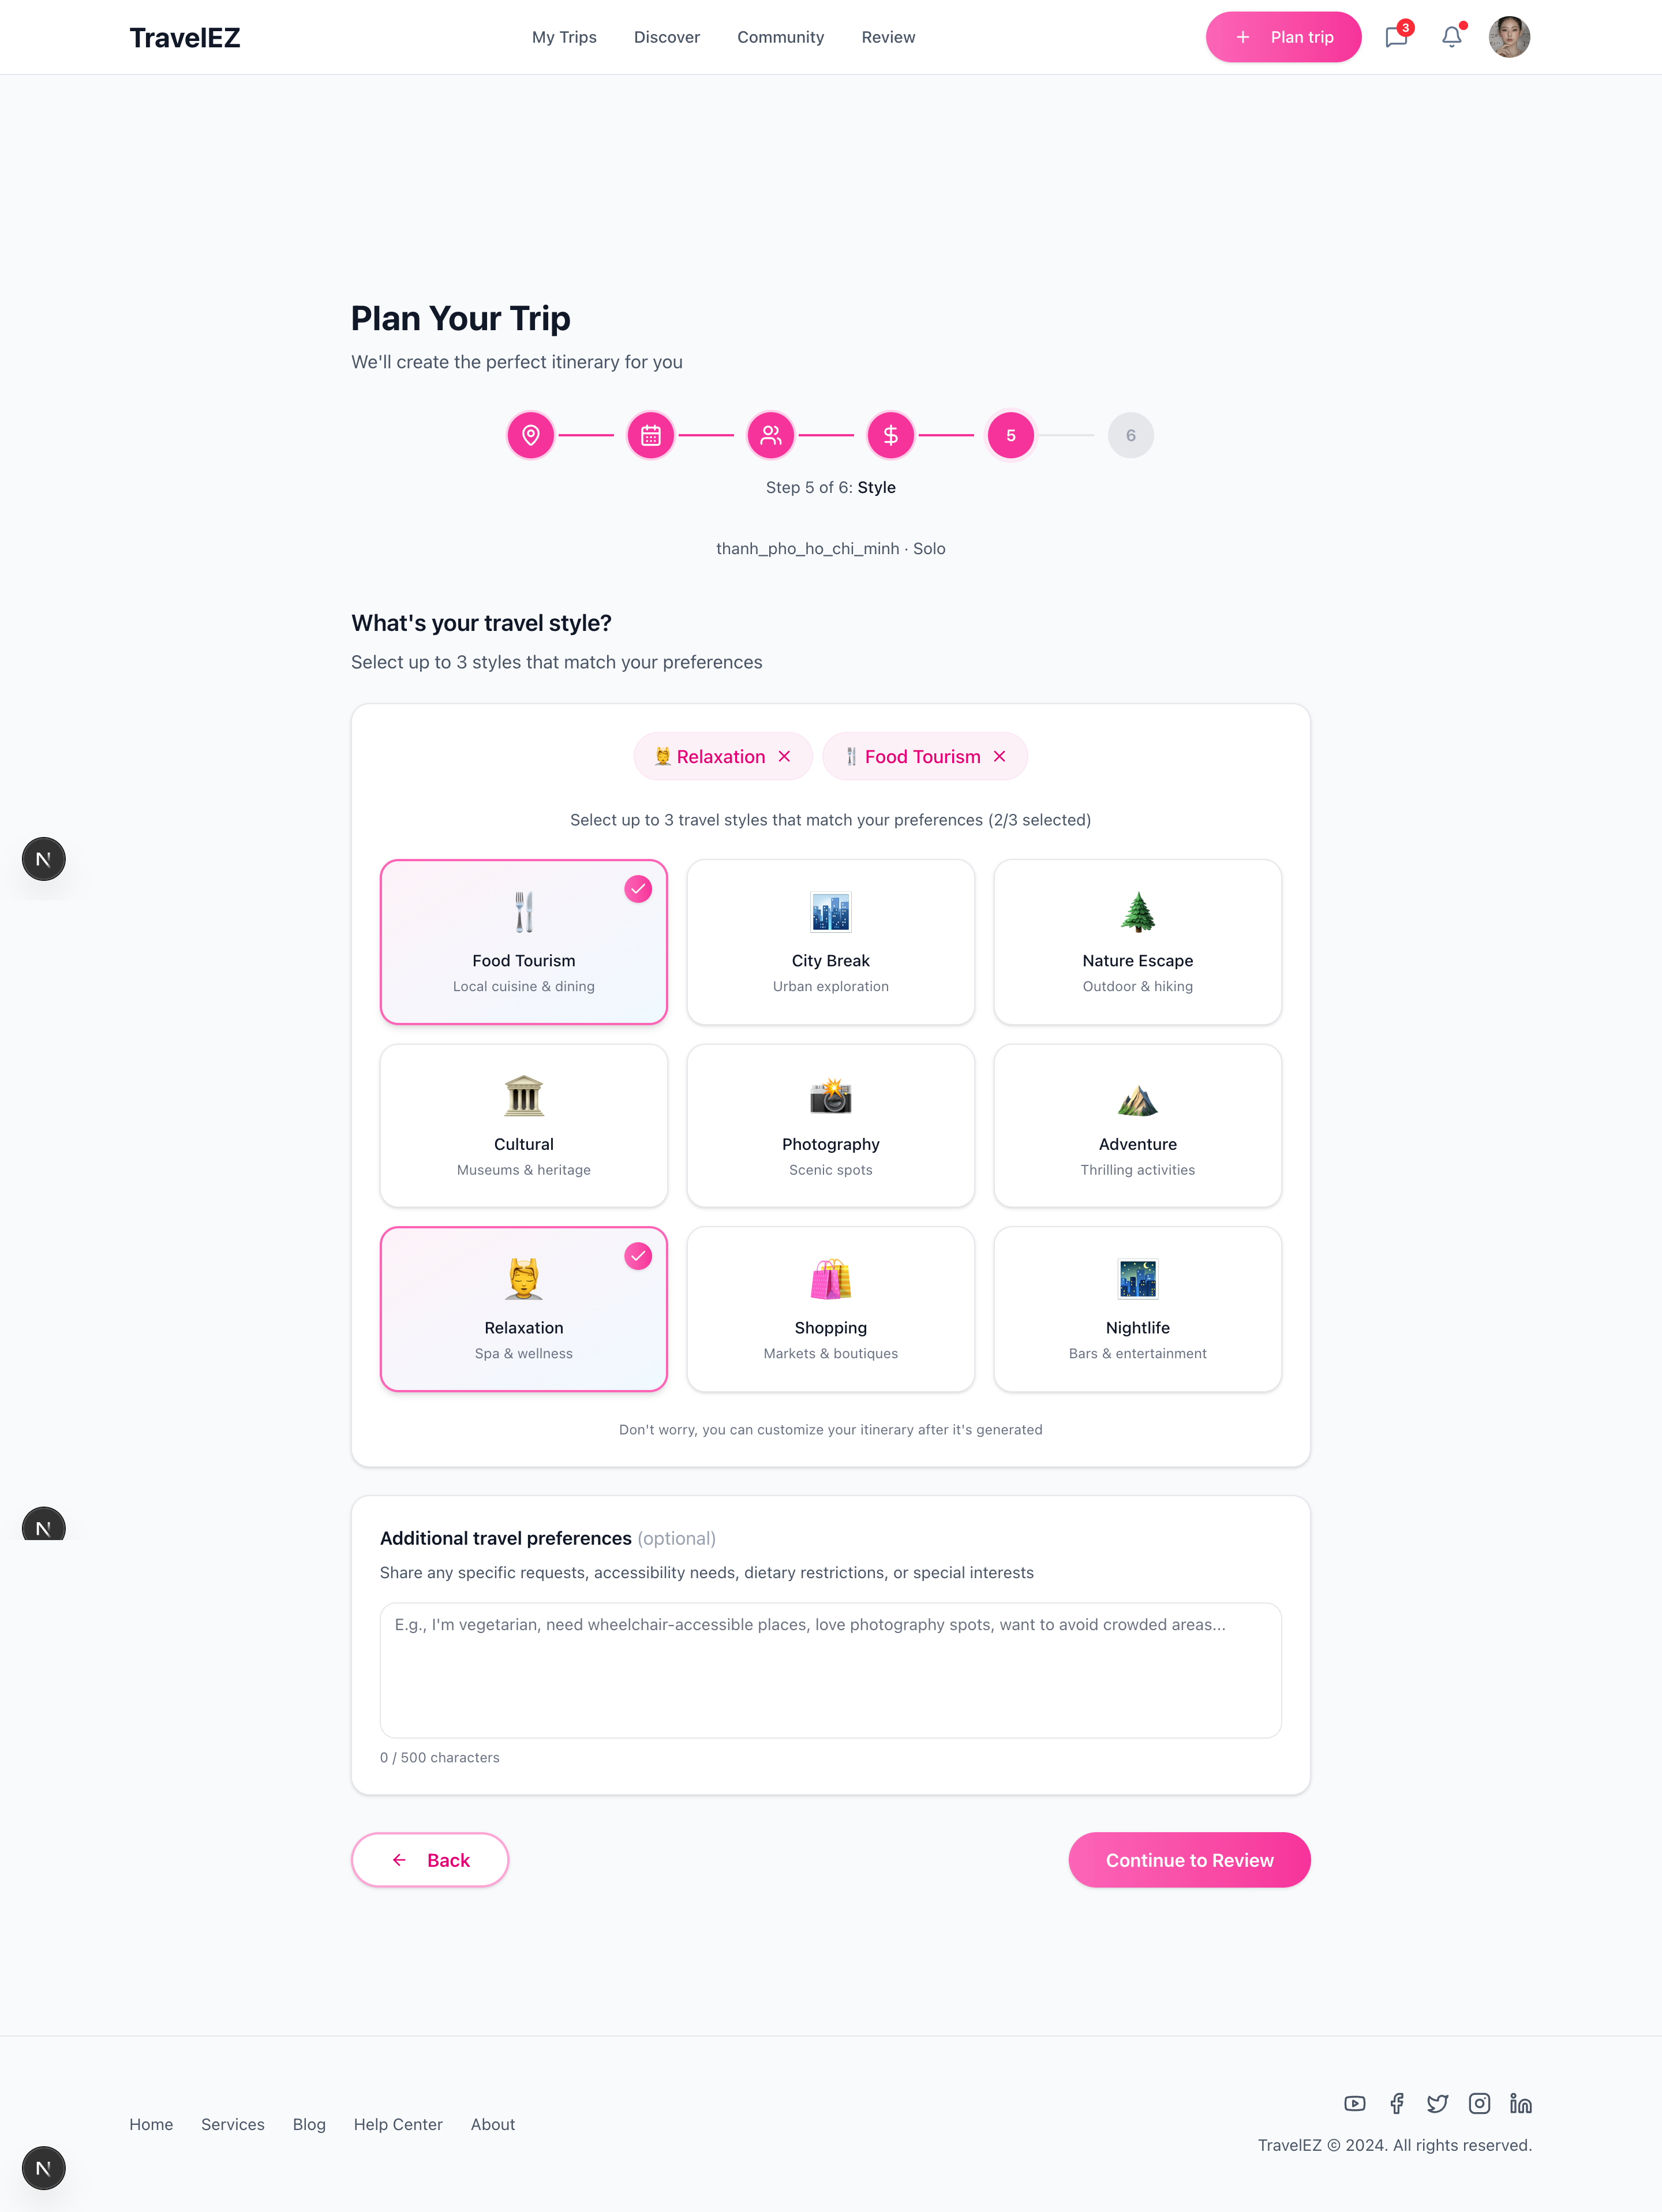
\includegraphics[
        width=1\textwidth
    ]{Images/7. System Design/UI design/planning-5.png}
    \caption{Trang lập kế hoạch chuyến đi bằng AI (bước 5 - Chọn sở thích)}
    \label{fig:planning-5}
\end{figure}

\begin{figure}[H]
    \centering
    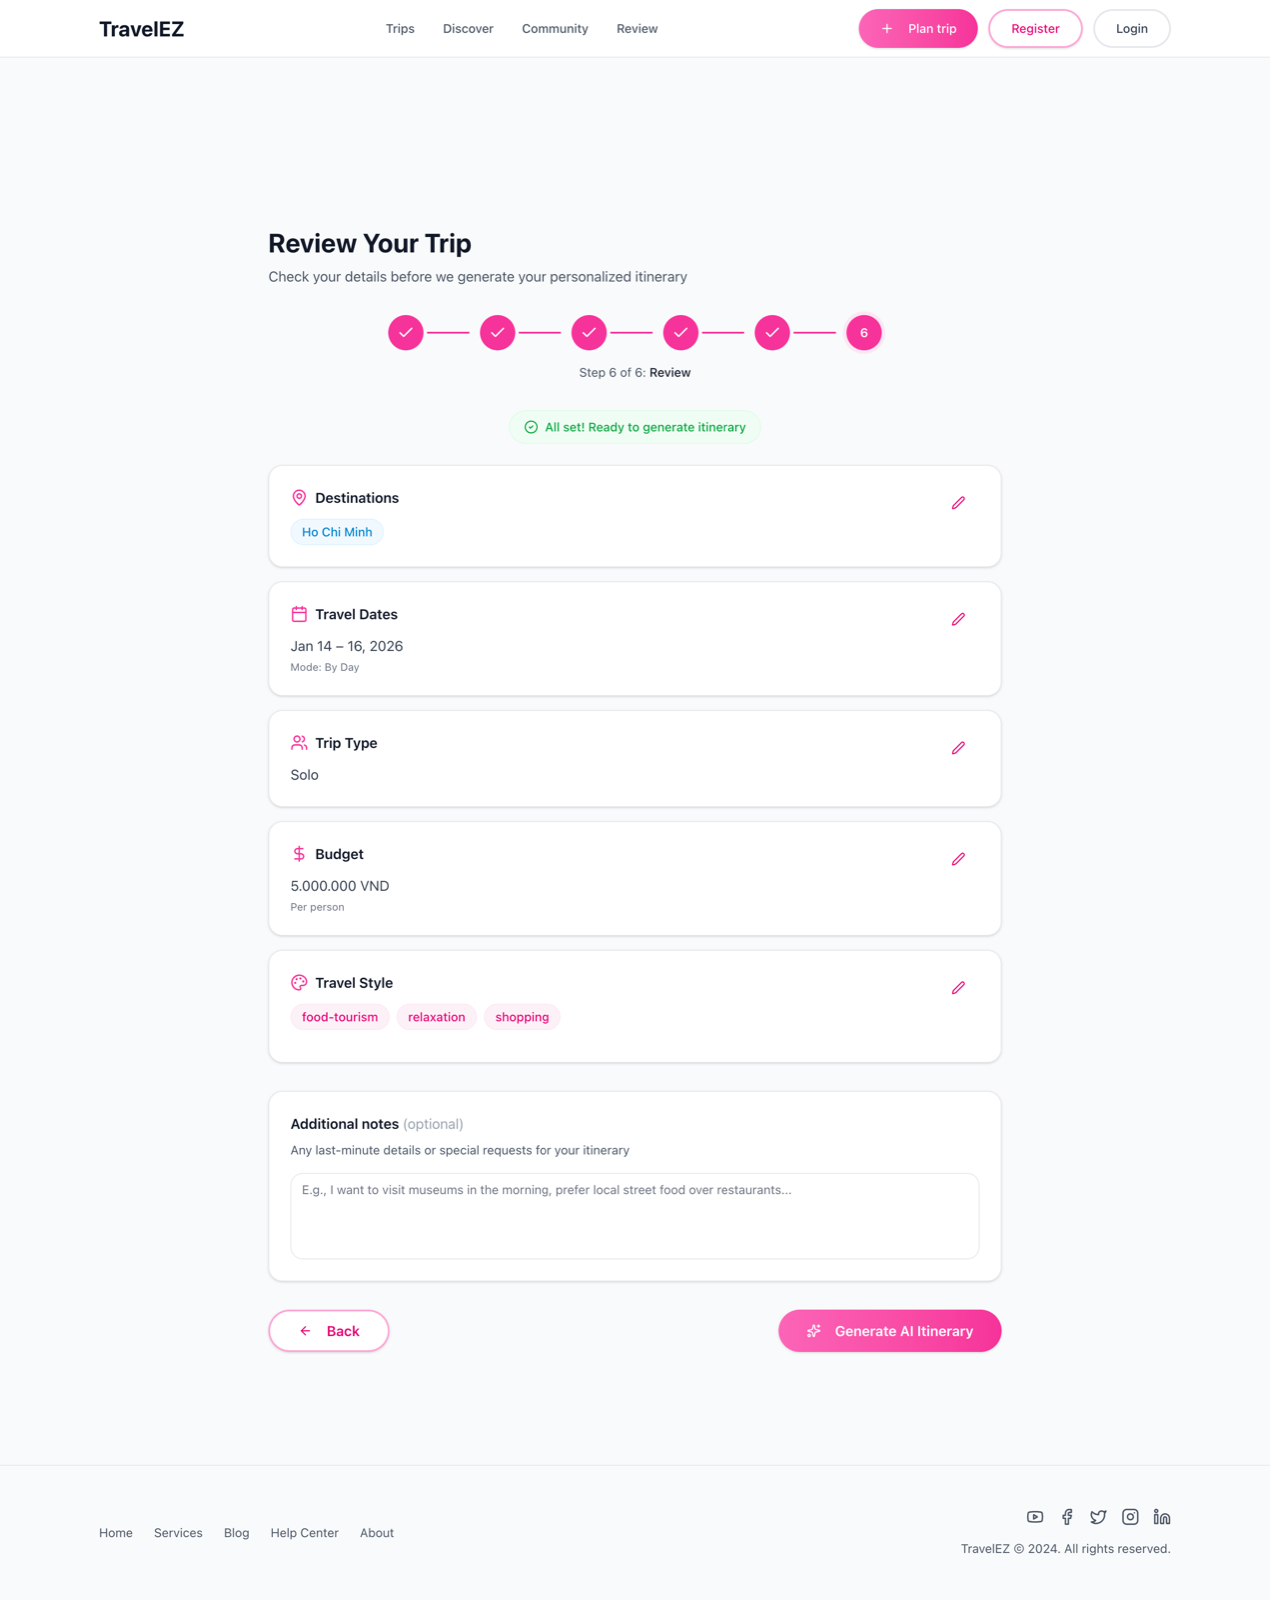
\includegraphics[
        width=1\textwidth
    ]{Images/7. System Design/UI design/planning-6.png}
    \caption{Trang lập kế hoạch chuyến đi bằng AI (bước 6 - Xác nhận)}
    \label{fig:planning-6}
\end{figure}

\begin{figure}[H]
    \centering
    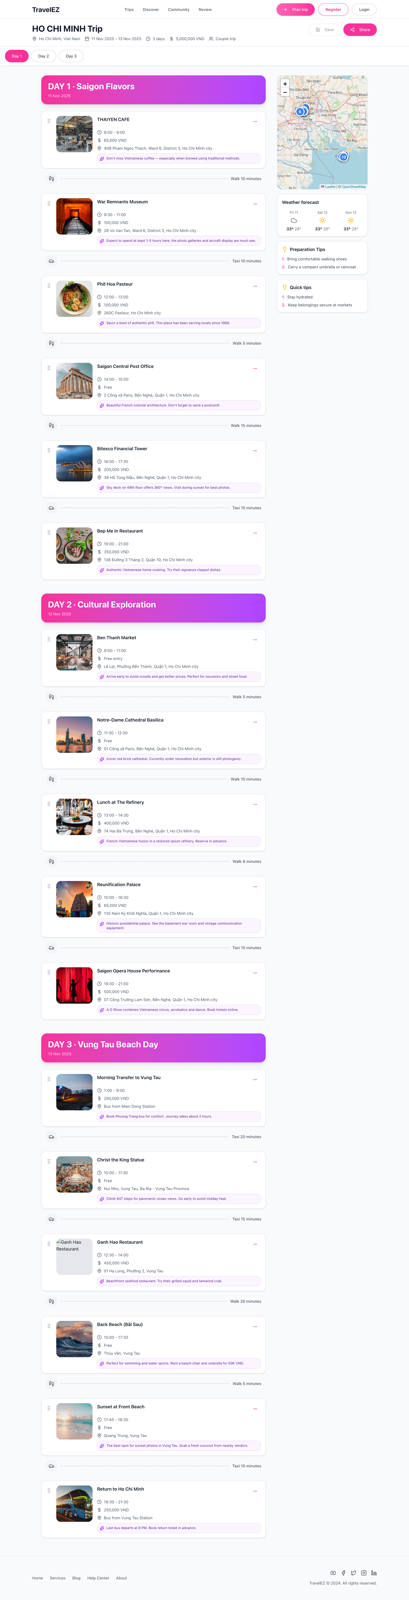
\includegraphics[
        height=1\textheight,
        keepaspectratio
    ]{Images/7. System Design/UI design/itinerary.png}
    \caption{Trang xem chi tiết lịch trình chuyến đi}
    \label{fig:itinerary}
\end{figure}

\begin{figure}[H]
    \centering
    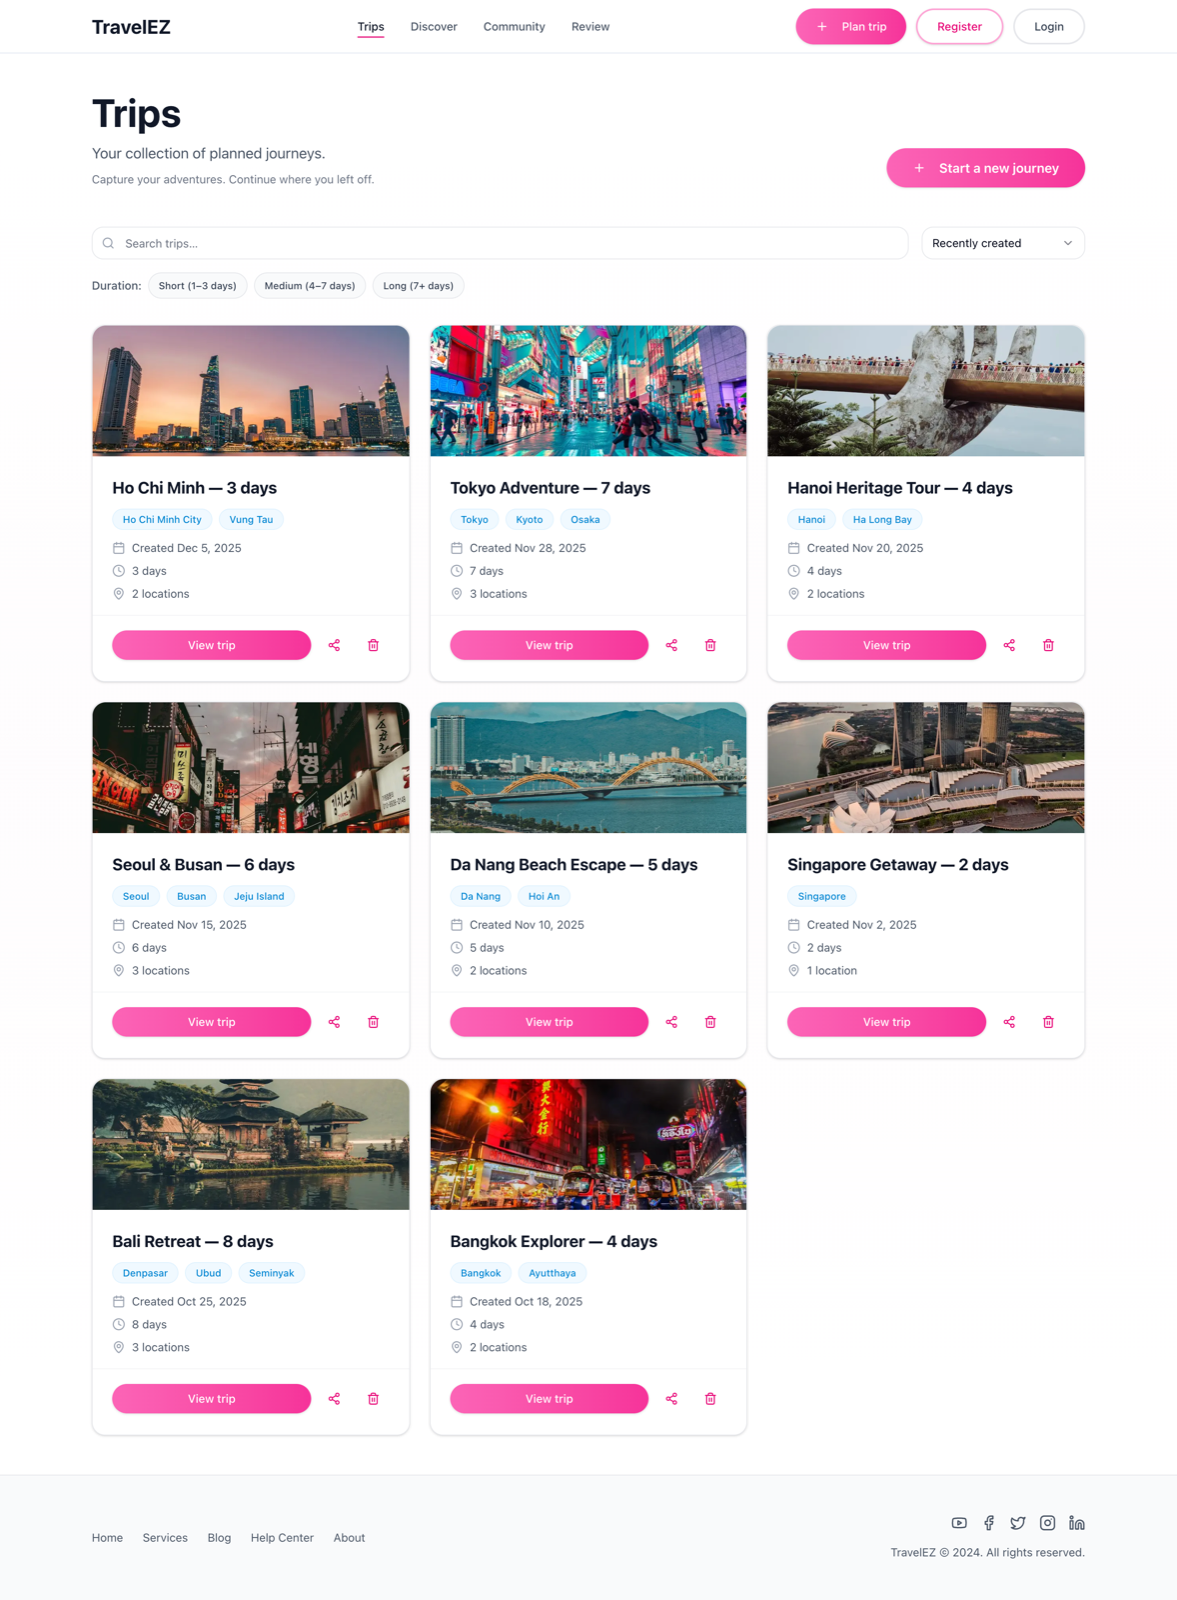
\includegraphics[
        width=1\textwidth
    ]{Images/7. System Design/UI design/trips.png}
    \caption{Trang quản lý các chuyến đi}
    \label{fig:trips}
\end{figure}

\begin{figure}[H]
    \centering
    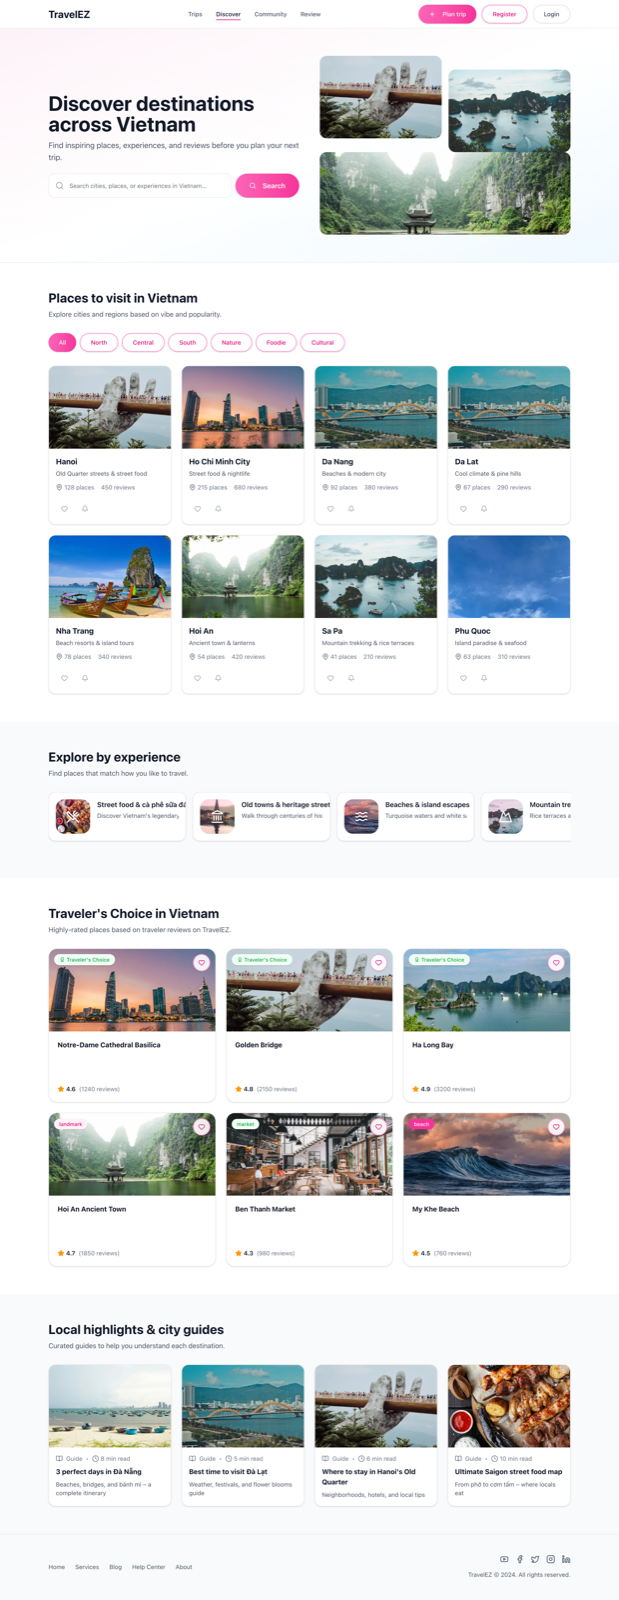
\includegraphics[
        height=1\textheight,
        keepaspectratio
    ]{Images/7. System Design/UI design/discovery.png}
    \caption{Trang khám phá điểm đến}
    \label{fig:discovery}
\end{figure}

\begin{figure}[H]
    \centering
    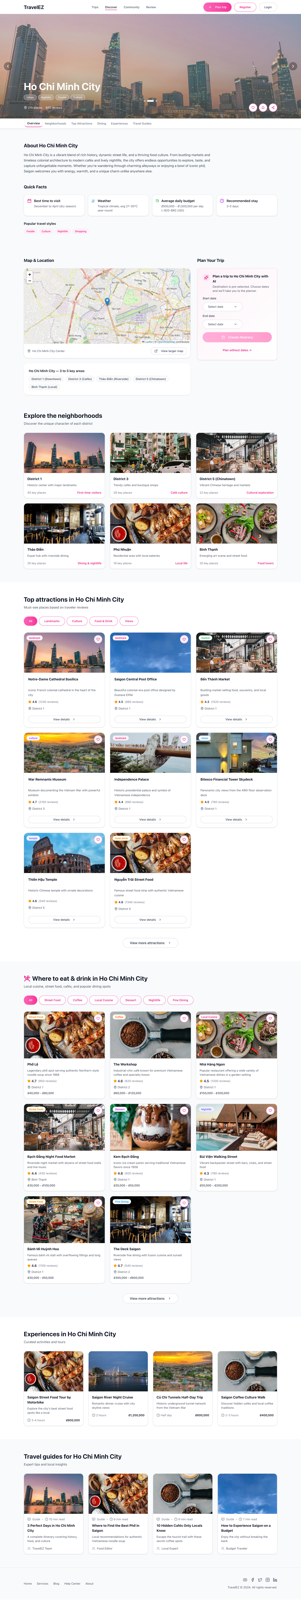
\includegraphics[
        height=1\textheight,
        keepaspectratio
    ]{Images/7. System Design/UI design/city.png}
    \caption{Trang danh sách địa điểm}
    \label{fig:city}
\end{figure}

\begin{figure}[H]
    \centering
    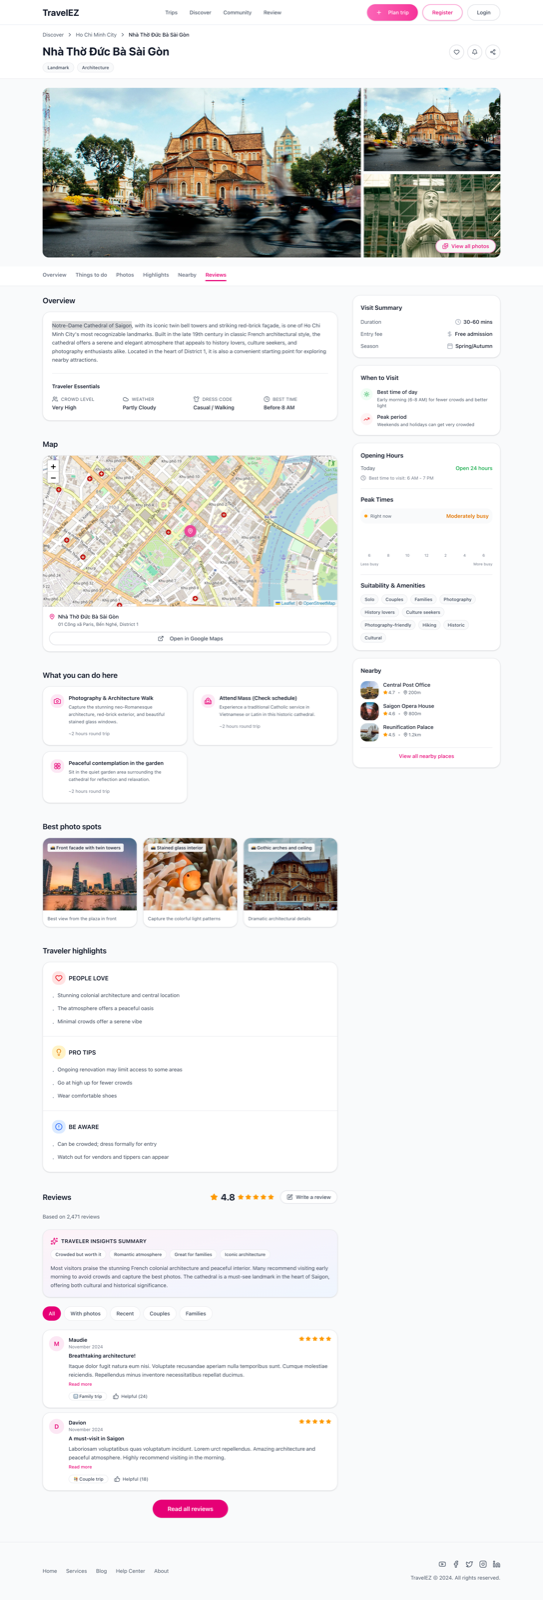
\includegraphics[
        height=1\textheight,
        keepaspectratio
    ]{Images/7. System Design/UI design/poi.png}
    \caption{Trang chi tiết địa điểm}
    \label{fig:poi}
\end{figure}

\begin{figure}[H]
    \centering
    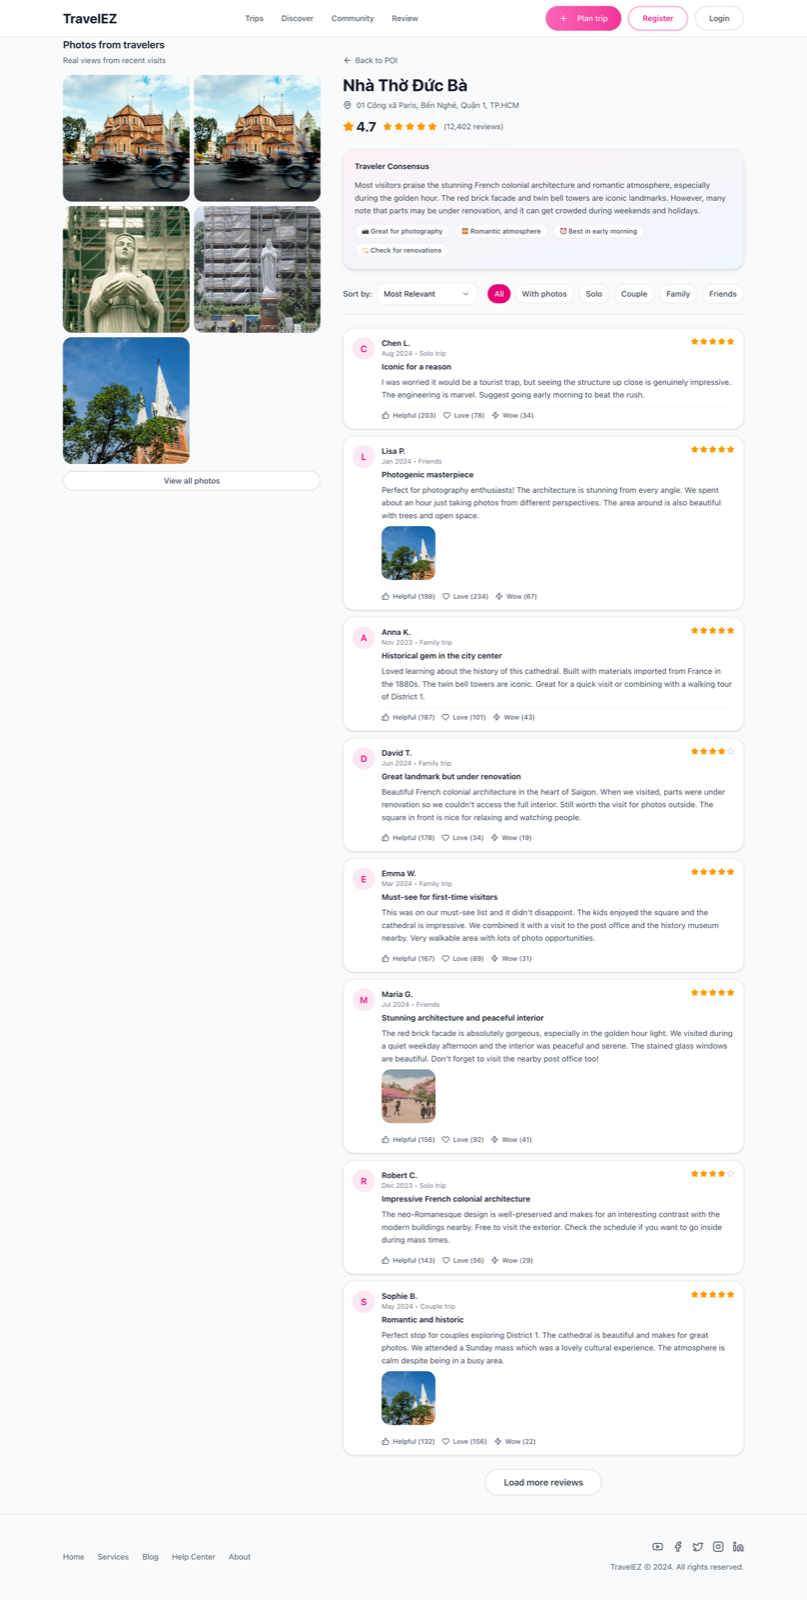
\includegraphics[
        width=0.7\textwidth
    ]{Images/7. System Design/UI design/review.png}
    \caption{Trang đánh giá}
    \label{fig:review}
\end{figure}
